\section{Future Work}

Our end-to-end \gls{nn} pipeline shows significant fallbacks on human cropping---the proposed method of introducing cropping to improve accuracies has been shown to degrade our performance, rather than the initial intention to improve it (\cref{sec:evaluation:results}). Overcoming this limitation may be as simple as re-training \frcnn{} simply on cropped images with wider padding, rather than on raw images, though testing such a hypothesis is left open.

While we have developed a system to label the prominence of runners, we still leave the implementation of a classifier to understand what prominence is open to future work. By proposing a method by which all crowded photos are discarded and teaching a classifier on biased \glsx{lop} (i.e., by removing the intermediary \textsc{maybe} candidates), such prominence ranking of subjects is within reach.

Similarly, the degrading text area detection may be improved by applying transfer learning to other \gls{rcnn}-based networks on a per-pixel level. As mentioned in \cref{sec:background:detection:learning}, Mask-\gls{rcnn}, has recently appeared as a preprint in early \citeyear{He:2017ud}. Improvements to Argus to record data points on a per-pixel basis may allow for improvement in the areas of per-pixel detection, thereby extracting digits from an \gls{rbn} within a bib even easier. An illustration of potential applications are shown in \cref{fig:conclusion:future_work:mask_rcnn}.

We propose to mitigate the bottleneck limitation of poor character detection by applying transfer learning to \frcnn{} in a similar fashion to that described in \cref{sec:processing_pipeline:bib_detection:deep_learning}. By producing a synthetic \gls{rbn} dataset similar to that of \citet{Jaderberg:2014uy,Jaderberg:2016wj} (with ground truth bounding boxes of each character known), we can augment these sample \glspl{rbn} and therefore re-train \frcnn{} to understand positions of characters. Each character from the detected regions can be extracted and piped into a \gls{cnn} trained on recognising specific digits, or perhaps---in addition to training \frcnn{} to learn the positions of characters---the characters themselves can be trained in the same process. We leave such an implementation open to future works.

\begin{figure}
  \centering
  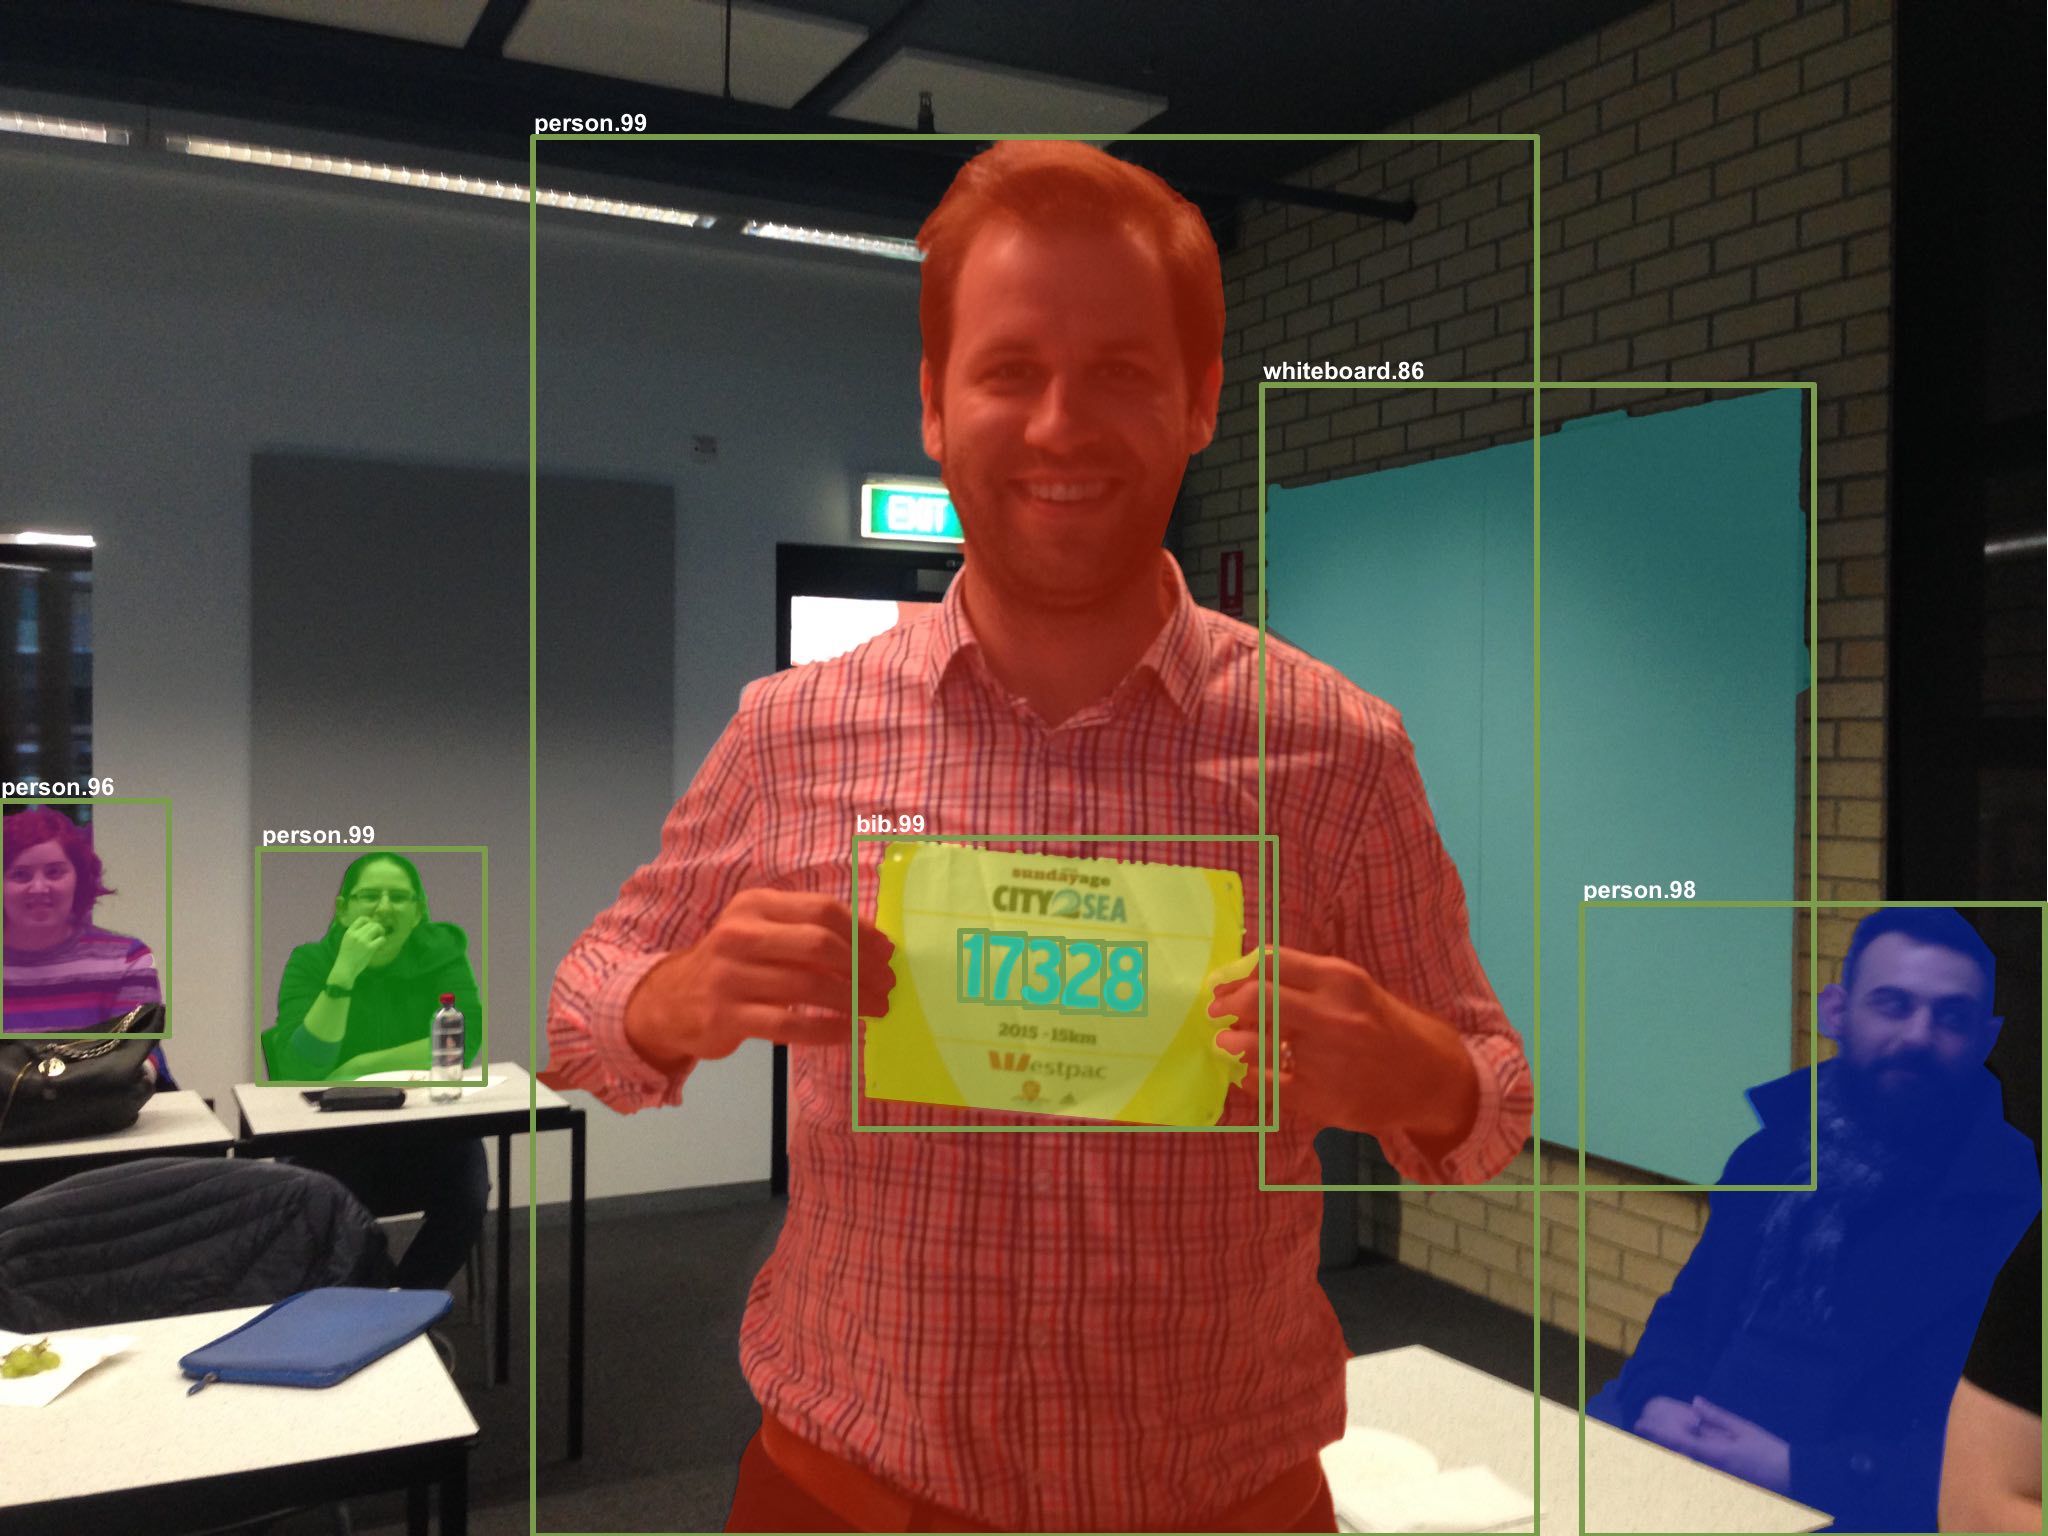
\includegraphics[width=0.9\textwidth]{images/conclusion/mask-rcnn}
  \caption[Potential use of Mask-RCNN on to recognise an RBN]{Potential use of Mask \gls{rcnn} to detect a bib sheet and its \gls{rbn} on with per-pixel accuracy.}
  \label{fig:conclusion:future_work:mask_rcnn}
\end{figure}